\documentclass{article}
\usepackage{fontspec}
\usepackage{xeCJK}
\setCJKmainfont[AutoFakeBold=2]{SimSun}
%\setCJKsansfont{SimHei}
\usepackage{amsmath, amssymb, amsthm}
\usepackage{geometry}
\usepackage{tikz}
\usepackage{fancyhdr}
\usepackage{tablefootnote}
%\setlength{\headheight}{15pt}
\usetikzlibrary{calc, intersections} % ABX 用於某些符號，若無可刪除
\usepackage{enumitem}
\usepackage{tkz-euclide}
\usepackage{zhnumber}
\newcommand{\INDEX}[1]{\fbox{\textbf{#1}}\ }
%\setlength{\headheight}{15pt} % 避免頁首高度警告
\setlength{\parskip}{1em}
\geometry{
  left=2.5cm, 
  right=2.5cm, 
  top=2.5cm, 
  bottom=2.5cm
}

% 設定頁首頁尾
\pagestyle{fancy}
%\fancyhf{}
\renewcommand{\headrulewidth}{2pt}
\renewcommand{\footrulewidth}{2pt}
\lhead{廖汶鋒}
\chead{綜合能力測評}
\rhead{澳門培道中學}
\fancyfoot[C]{\thepage} % Centered footer
\fancyfoot[L]{\zhtoday} % Left footer

\title{\textbf{綜合能力測評（題目）}\vspace{-0.5em}}
\author{澳門培道中學　廖汶鋒}
\date{\zhtoday}
\linespread{1.3}

% 設定段落首行縮進
\setlength{\parindent}{0em}

\begin{document}
%\thispagestyle{fancy}  % 讓首頁也顯示頁首
\maketitle
%{
%\begin{center}
%  \textbf{\Large{能力測評題題目及答案}}
%\end{center}
%
如遇到困難時，不妨嘗試使用各種 AI 工具來協助解題，或是使用 GeoGebra 來繪製幾何圖形，這些工具都能幫助你更好地理解問題並找到解決方案。

%================ Problem 1 ================%
設$\Omega$與$\Gamma$分別是以後$M,N$為圓心的圓，且圓$\Omega$的半徑小於圓$\Gamma$的半徑。
設$\Omega$與$\Gamma$交於相異兩點$A,B$。直線$MN$與圓$\Omega$交於點$C$、與圓$\Gamma$交於點$D$，
且$C,M,N,D$四點依此順序落在該直線上。直線$AP$與圓$\Omega$交於點$E\neq A$、與圓$\Gamma$再交於點$F\neq A$。
令點$H$為$\triangle{PMN}$的垂心。\\[0.5em]
\textbf{求證：}通過$H$且平行於$AP$的直線$l$，與$\triangle{BEF}$的外接圓相切。

\begin{center} % p1示意圖
  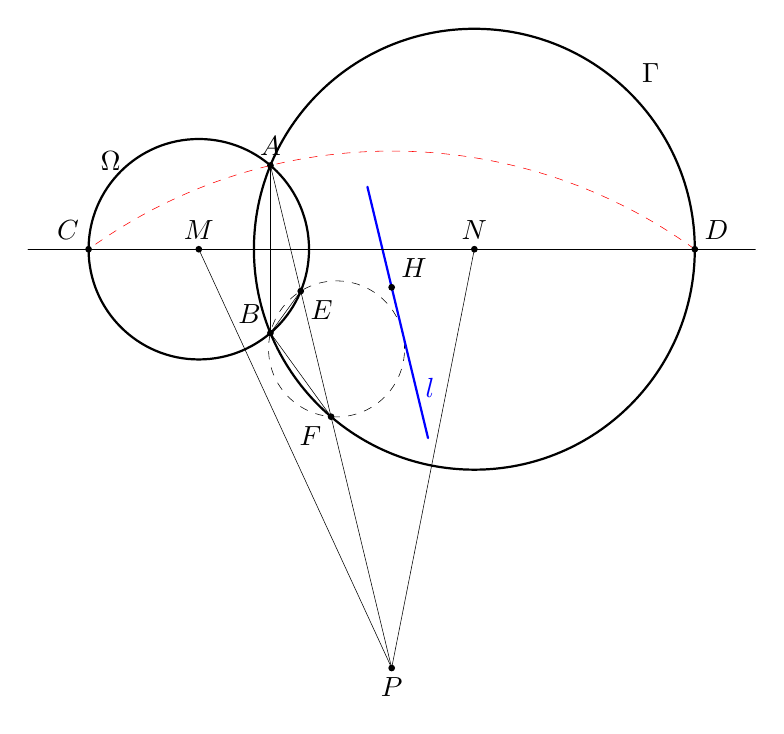
\begin{tikzpicture}[scale=0.7]
      % --- 1. 定義圓心 M, N 與半徑 ---
      \tkzDefPoint(-2,0){M}
      \tkzDefPoint(3,0){N}
      \def\rO{2}
      \def\rG{4}
      
      % --- 2. 定義直線 MN 上的 C, D (確保 C, M, N, D 順序) ---
      \tkzDefPoint(-2-\rO,0){C}
      \tkzDefPoint(3+\rG,0){D}
      
      % --- 3. 繪製兩圓 Omega, Gamma ---
      \tkzDrawCircle[thick,black](M,C)
      \tkzDrawCircle[thick,black](N,D)
      
      % --- 4. 求兩圓交點 A, B ---
      \tkzInterCC(M,C)(N,D) \tkzGetPoints{A}{B}
      
      % --- 5. 定義 P 為三角形 ACD 的外心 ---
      \tkzCircumCenter(A,C,D) \tkzGetPoint{P}
      %\tkzDrawCircle[dashed, cyan](P,A) % 繪製 ACD 的外接圓供參考
      \tkzDrawArc[color=red, dashed](P,D)(C)
      % --- 6. 構造割線 AP 並求交點 E, F ---
      \tkzInterLC(A,P)(M,C) \tkzGetPoints{E}{A_tmp}
      \tkzInterLC(A,P)(N,D) \tkzGetPoints{A_tmp2}{F}
      
      % --- 7. 計算三角形 PMN 的垂心 H ---
      \tkzOrthoCenter(P,M,N) \tkzGetPoint{H}
      
      % --- 8. 繪製三角形 BEF 的外接圓 ---
      \tkzCircumCenter(B,E,F) \tkzGetPoint{O_BEF}
      \tkzDrawCircle[dashed, black](O_BEF,B)
      
      % --- 9. 繪製通過 H 且平行於 AP 的切線 l ---
      \tkzDefLine[parallel=through H](A,P) \tkzGetPoint{l_dir}
      \tkzDrawLine[blue, thick, add=0.2 and -0.7](H,l_dir)
      
      % --- 10. 繪製線段與標籤 ---
      \tkzDrawLines[add=0.1 and 0.1](C,D)
      \tkzDrawSegments(A,P P,M P,N A,B B,E B,F)
      \tkzDrawPoints[fill=black](M,N,A,B,C,D,E,F,P,H)
      
      \tkzLabelPoints[above](M,N)
      \tkzLabelPoints[above left](C)
      \tkzLabelPoints[above right](D,H)
      \tkzLabelPoints[above left](B)
      \tkzLabelPoints[above](A)
      \tkzLabelPoints[below](P)
      \tkzLabelPoints[below right](E)
      \tkzLabelPoints[below left](F)
      
      \node at (-2-\rO*0.8,\rO*0.8) {$\Omega$};
      \node at (3+\rG*0.8,\rG*0.8) {$\Gamma$};
      \coordinate (l_1) at ($(H)!0.2!(l_dir)$);
      \node[blue, right] at (l_1) {$l$};

  \end{tikzpicture}
\end{center} 
%================ Problem 1 ================%
\newpage
%================ Problem 2 ================%
設四邊形$ABCD$是梯形，$AB\parallel CD$且$AB<CD$。
直線$AD$和$BC$交於點$P$。$\triangle{ABC}$上的一點$X\neq C$滿足$PX=PC$，
$\triangle{ABD}$上的一點$Y\neq D$滿足$PY=PD$直線$AX$與$BY$交於點$Q$。

\textbf{求證：}$PQ\parallel AB$
\begin{center} % p2 示意圖
  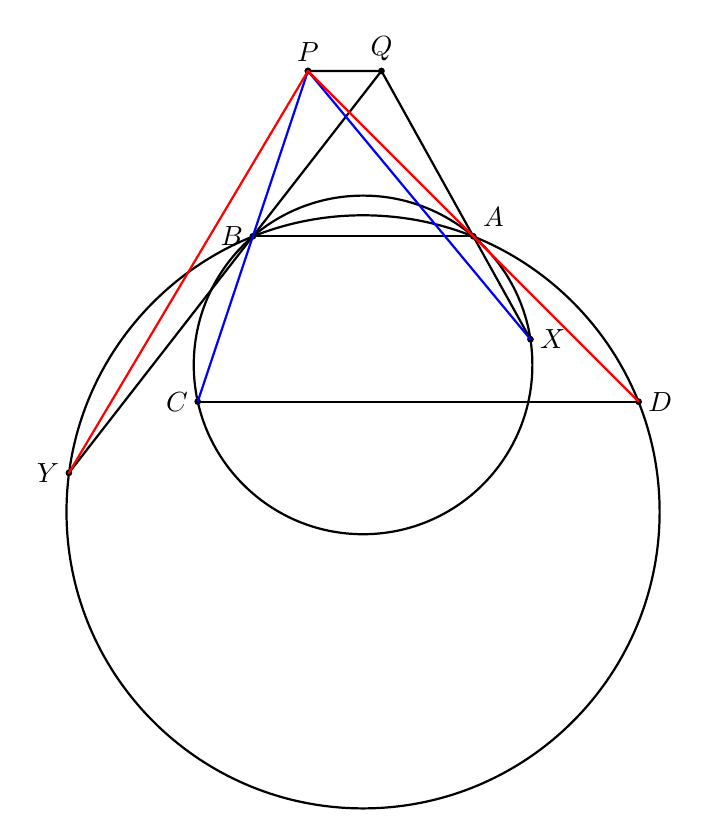
\begin{tikzpicture}[scale=0.7]
    \tkzDefPoint(2,3){A}
    \tkzDefPoint(-2,3){B}
    \tkzDefPoint(-3,0){C}
    \tkzDefPoint(5,0){D}
    \tkzInterLL(A,D)(B,C) \tkzGetPoint{P}
    \tkzCircumCenter(A,B,C) \tkzGetPoint{O_1}
    \tkzCircumCenter(A,B,D) \tkzGetPoint{O_2}
    \tkzInterCC(O_1,C)(P,C) \tkzGetPoints{C_tmp}{X}
    \tkzInterCC(O_2,D)(P,D) \tkzGetPoints{Y}{D_tmp}
    \tkzDrawCircle[black,thick](O_1,A)
    \tkzDrawCircle[black,thick](O_2,A)
    \tkzInterLL(A,X)(B,Y) \tkzGetPoint{Q}
    \tkzDrawPoints[fill=black](A,B,C,D,P,X,Y,P,Q)
    \tkzLabelPoints[right](D)
    \tkzLabelPoints[above right](A)
    \tkzLabelPoints[left](B,C)
    \tkzLabelPoints[above](P)
    \tkzLabelPoints[above](Q)
    \tkzLabelPoints[right](X)
    \tkzLabelPoints[left](Y)
    \tkzDrawSegments[black, thick](A,B C,D P,Q X,Q Y,Q)
    \tkzDrawSegments[blue, thick](P,X P,C)
    \tkzDrawSegments[red, thick](P,Y P,D)
  \end{tikzpicture}
\end{center}
%================ Problem 2 ================%
\newpage
%================ Problem 3 ================%
滿足下列條件 (i) 和 (ii) 的有限長實數列 $\left\{a_n\right\}_{n=1}^{m}\left(m\geq10\right)$ 是一個 $m$-有趣數列：
\begin{enumerate}[label = (\roman*)]
  \item 對任意 $k=1,2,\cdots,m-1$，都有 $\left|a_{k+1}-a_k\right|=1$；
  \item 存在正整數 $i_1,i_2,\cdots,i_{10}\left(i_1<i_2<\cdots<i_{10}\leq m\right)$，使得 $\left\{a_{i_k}\right\}_{k=1}^{10}$ 是等比數列，且該等比數列的公比 $q\neq\pm1$。
\end{enumerate}
記 $m_0$ 為使得 $m$-有趣數列存在的最小正整數 $m$。求 $m_0$ 的值，並確定不同的 $m_0$-有趣數列的個數。
%================ Problem 3 ================%
\newpage
%================ Problem 4 ================%
不等邊銳角 $\triangle{ABC}$ 的外心為 $O$，
由 $A$ 點向 $BC$ 的垂線的垂足為 $D$，
$P$ 點在直線 $AO$ 上且不在 $\triangle{ABC}$ 的外接圓上。
以線段 $AP$ 為直徑的圓$\Gamma$，與 $\triangle{BCP}$ 的外接圓相交於 $E\neq P$，
與平行於 $BC$ 且過 $A$ 的直線相交於 $F\neq A$。

\textbf{求證：}$D$、$E$ 和 $F$ 三點共線。
\begin{figure}[htbp] % p4 示意圖
  \centering
  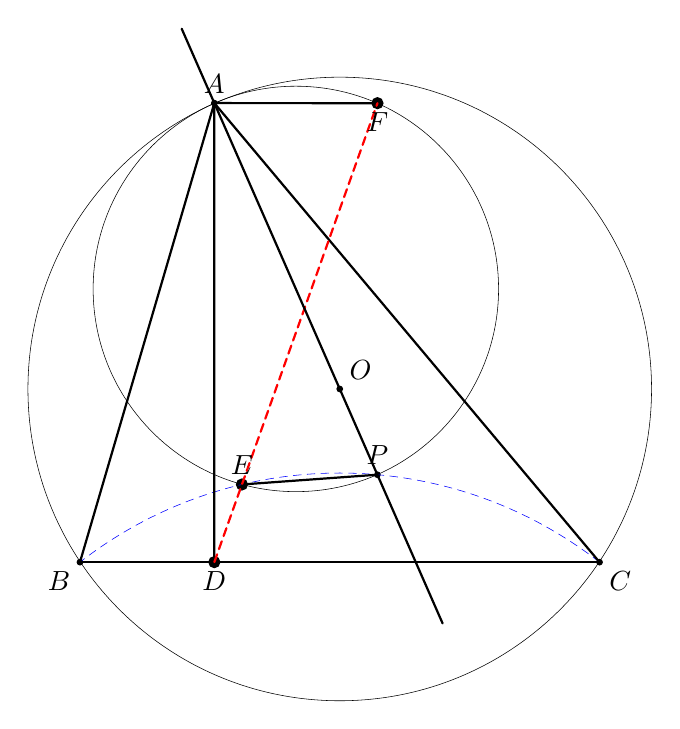
\begin{tikzpicture}[scale=1.1]
    \tkzDefPoints{0/0/O, -3/-2/B, 3/-2/C}
    \tkzDefPointBy[rotation=center O angle -100](B)\tkzGetPoint{A}
    \tkzDefPointBy[projection=onto B--C](A)\tkzGetPoint{D}
    \tkzDefPointWith[linear, K=1.3](A,O)\tkzGetPoint{P}
    \tkzDefPointWith[linear, K=0.5](A,P)\tkzGetPoint{X}
    \tkzDefCircle[circum](B,P,C)\tkzGetPoint{O1}
    \tkzInterCC[common=P](X,P)(O1,P)\tkzGetFirstPoint{E}
    \tkzDefLine[parallel=through A](B,C)\tkzGetPoint{L}
    \tkzInterLL(A,L)(D,E)\tkzGetPoint{F}
    \tkzDrawPoints[black](A,B,C,P,O)
    \tkzDrawPoints[size=4, fill=black](D,E,F)
    \tkzDrawCircle[black](O,B)
    \tkzDrawCircle[black](X,A)
    \tkzDrawArc[blue, densely dashed](O1,C)(B)
    \tkzDrawSegments[black, thick](A,B A,C B,C A,D P,E A,F)
    \tkzDrawSegment[red, thick, densely dashed](D,F)
    \tkzDrawLine[black, thick, add=0.2 and 0.4](A,P)
    \tkzLabelPoints[above](A,E,P)
    \tkzLabelPoints[below left](B)
    \tkzLabelPoints[below right](C)
    \tkzLabelPoints[below](D,F)
    \tkzLabelPoints[above right](O)
  \end{tikzpicture}
\end{figure}
%================ Problem 4 ================%
\newpage
%================ Problem 5 ================%
\INDEX{問題 5}$\triangle{ABC}$ 的重心為 $G$，$R$ 和 $S$ 分別在射線 $GB$ 和 $GC$ 上，且滿足
$$
  \angle{ABS}=\angle{ACR}=180^{\circ}-\angle{BGC}
$$
\textbf{求證：}$\angle{RAS}+\angle{BAC}=\angle{BGC}$。
\begin{figure}[htbp] % p5 示意圖
  \centering
  \begin{tikzpicture}[scale=1.1]
    \tkzDefPoints{-0.5/7/A, -2/0/B, 3/0/C}
    \tkzDefTriangleCenter[centroid](A,B,C)\tkzGetPoint{G}
    \tkzDefLine[orthogonal=through B](A,B)\tkzGetPoint{X1}
    \tkzDefLine[mediator](G,B)\tkzGetPoints{X2}{X3}
    \tkzInterLL(B,X1)(X2,X3)\tkzGetPoint{O_B}
    \tkzInterLC[common=G](G,C)(O_B,G)\tkzGetFirstPoint{S}
    \tkzDefLine[orthogonal=through C](A,C)\tkzGetPoint{Y1}
    \tkzDefLine[mediator](G,C)\tkzGetPoints{Y2}{Y3}
    \tkzInterLL(C,Y1)(Y2,Y3)\tkzGetPoint{O_C}
    \tkzInterLC[common=G](G,B)(O_C,G)\tkzGetFirstPoint{R}
    \tkzDrawPoints[black](A,B,C,G,R,S)
    \tkzDrawSegments[black, thick](A,B A,C B,C G,R G,S B,S C,R)
    %\tkzDrawCircles[black, thick](O_B,G O_C,G)
    \tkzLabelPoints[above](A,G)
    \tkzLabelPoints[left](B,R)
    \tkzLabelPoints[right](C,S)
    \tkzMarkAngle[size=0.4, color=blue, line width=1.5pt](S,B,A)
    \tkzMarkAngle[size=0.4, color=blue, line width=1.5pt](A,C,R)
    \tkzMarkAngle[size=0.4, color=red, line width=1.5pt](B,G,C)
  \end{tikzpicture}
\end{figure}
%================ Problem 5 ================%
\end{document}